\documentclass{beamer}
\usepackage[utf8]{inputenc}
\usepackage{graphics}
\mode<presentation> {
\usetheme{unc}}
\setbeamertemplate{navigation symbols}{} % To remove the navigation symbols from the bottom of all slides uncomment this line

\usepackage{graphicx} % Allows including images
\usepackage{booktabs} % Allows the use of \toprule, \midrule and \bottomrule in tables


\usepackage{hyperref}
\hypersetup{linkcolor=blue,colorlinks=true}


% Remove symbols
\beamertemplatenavigationsymbolsempty


%\usetheme{default}

\usefonttheme{serif}

%----------------------------------------------------------------------------------------
%	TITLE PAGE
%----------------------------------------------------------------------------------------


\title[The Puzzle of War (I)]{\LARGE{The Puzzle of Interstate War, Part I: Conflict as Bargaining}}
\author[POLI 150]{Steven Saroka}
\institute{POLI 150}
\date{25 January 2023}


\begin{document}

\begin{frame}
\titlepage % Print the title page as the first slide
\end{frame}


%\begin{frame}
%\frametitle{Overview} % Table of contents slide, comment this block out to remove it
%\tableofcontents % Throughout your presentation, if you choose to use \section{} and \subsection{} commands, these will automatically be printed on this slide as an overview of your presentation
%\end{frame}


%%% SLIDE TEMPLATES

% Template for images
% \begin{frame}{\LARGE Kurdistan}
%     \centering
% \includegraphics[width=\textwidth,height=0.8\textheight,keepaspectratio]{}
% \end{frame}

% %% Core template for the slides
% \begin{frame} 
% \frametitle{\LARGE{}}
% \end{frame}

%----------------------------------------------------------------------------------------
%	PRESENTATION SLIDES
%----------------------------------------------------------------------------------------


%% Slide outline
\begin{frame} 
	\frametitle{\LARGE{Today's Class}}
	\begin{itemize}
		\Large{
			\item How to Read Academic Articles
			\\~\\ 
			\item Conflict as Bargaining
		}
	\end{itemize}
\end{frame}

\begin{frame} 
	\frametitle{\LARGE{Academic Article Layout}}
	Components of an academic article:
	\begin{itemize}
		\item Abstract
		\item Literature Review
		\item Theory/Hypotheses
		\item Methods
		\item Results
		\item Discussion
	\end{itemize}
	These elements are present in many articles you will read for this class.
\end{frame}

\begin{frame} 
	\frametitle{\LARGE{Academic Article Layout}}
	\begin{itemize}
		\item \textbf{Abstract}: Brief summary of main theoretical contribution and findings. \pause
		\item \textbf{Introduction}: Introduces relevant questions driving research. \pause
		\item \textbf{Literature Review}: Relevant prior work which influenced this work. \pause
		\item \textbf{Theory/hypotheses}: Author's proposed explanation for phenomena of interest and expected findings. \pause
		\item \textbf{Methods}: How the author is testing their hypotheses. \pause
		\item \textbf{Results}: What they found. \pause
		\item \textbf{Discussion}: Summary, potential weaknesses and future research directions. 
	\end{itemize}
\end{frame}

\begin{frame} 
	\frametitle{\LARGE{Academic Article Layout}}
	\begin{itemize}
		\item \textbf{Abstract}: Good for a brief summary/refresher. \pause
		\item \textbf{Introduction}: Useful for getting an idea of the paper. \pause
		\item \textbf{Literature Review}: Can be skipped (in this class). \pause
		\item \textbf{Theory/hypotheses}: Important to understand! \pause
		\item \textbf{Methods}: Can be skipped (in this class). \pause
		\item \textbf{Results}: Have a general idea of what this says, but don't get stuck in the details. \pause
		\item \textbf{Discussion}: Often useful as a summary of key findings. 
	\end{itemize}
\end{frame}

\begin{frame} 
	\frametitle{\LARGE{Central Question}}
	\begin{center}
		\LARGE Given the massive costs of war, why do states fight? 
	\end{center}
\end{frame}

\begin{frame} 
	\frametitle{\LARGE{Key Terms}}
	\begin{itemize}
		\item War 
		\item Interstate War
		\item Crisis Bargaining
		\item Status Quo
	\end{itemize}
\end{frame}

\begin{frame} 
	\frametitle{\LARGE{Battle of Stalingrad}}	
	\centering
	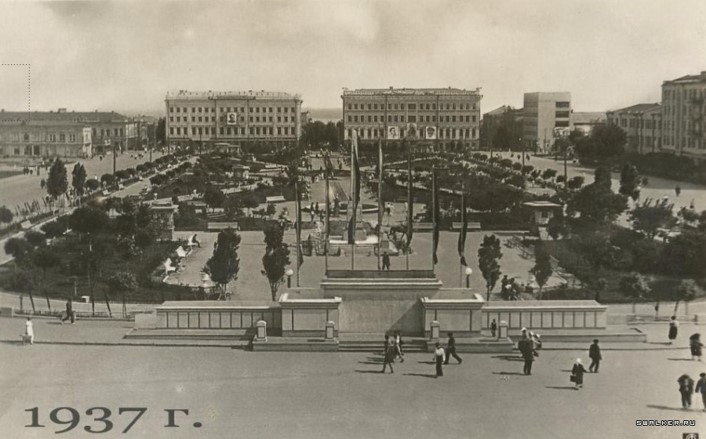
\includegraphics[width=\textwidth,height=0.85\textheight,keepaspectratio]{Stalingradpre.jpg}
\end{frame}

\begin{frame} 
	\frametitle{\LARGE{Battle of Stalingrad}}	
	\centering
	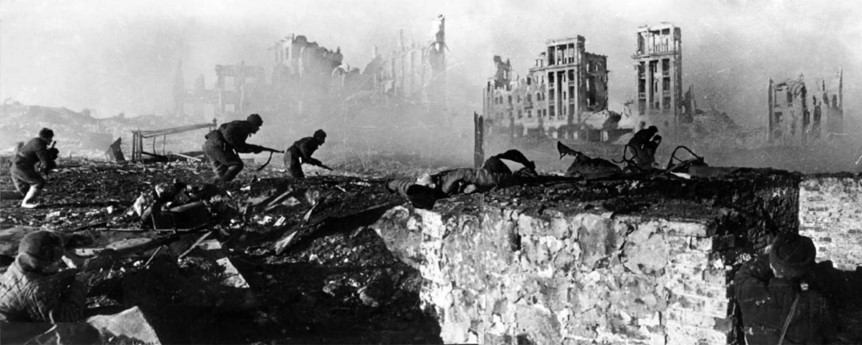
\includegraphics[width=\textwidth,height=0.9\textheight,keepaspectratio]{Stalingrad.jpg}
	\tiny Source:  https://www.britannica.com/summary/Battle-of-Stalingrad
\end{frame}

\begin{frame} 
	\frametitle{\LARGE{Battle of Stalingrad}}	
	\begin{itemize}
		\item July 1942 - February 1943
		\item German offensive intended to capture Stalingrad turns into grinding urban warfare. Soviet forces eventually triumph. \pause
		\item Estimated casualties: 
		\begin{itemize}
			\item 740,000 Axis casualties. \pause
			\item 790,000 Soviet casualties. \pause
		\end{itemize}
		\item 1.5 million combined casualties (for a low estimate!) \pause
		\item This seems like a terrible way to settle disputes.
	\end{itemize}
\end{frame}

\begin{frame} 
	\frametitle{\LARGE{Class Activity}}	
		\begin{center}
		\LARGE Define ``war"  without looking at the next slide!
	\end{center}
\end{frame}

%https://correlatesofwar.org/data-sets/COW-war/inter-state-wars-codebook
\begin{frame} 
	\frametitle{\LARGE{What is War Anyway?}}
	\begin{itemize}
		\item What is a reasonable definition of war? \pause
		\item Components of a war: \pause
		\begin{itemize}
			\item Violence \pause
			\item At least 2 clear sides \pause
			\item Some minimum amount of loss of life \pause
		\end{itemize}
		\item \textbf{War}: ``must involve sustained combat, involving organized armed forces, resulting in a minimum of 1,000 battle-related combatant fatalities within a twelve month period" (CoW Interstate Wars Codebook pg. 1) \pause
			\begin{itemize}
			\item Both sides must be capable of ``effective resistance" \pause
			\end{itemize}
		\item Most IR definitions of war are built on or just use this definition.
	\end{itemize}
\end{frame}

\begin{frame} 
	\frametitle{\LARGE{War Definition Implications}}
	Under this definition, which of the following are wars? \pause
	\begin{itemize}
		\item \textbf{Rwandan genocide}? \pause No, because Tutsi victims were not organized or able to effectively resist Hutu militias. \pause
		\item \textbf{Cartel and gang violence}? \pause No, not ``organized" like regular state military units. \pause
		\item \textbf{9/11}? \pause No, because no sustained combat, no organized armed forces, and few or no combatant fatalities (depending on whether terrorists are classed as combatants). \pause	
	\end{itemize}
	Note that this definition excludes these kinds of violence.
\end{frame}

\begin{frame} 
	\frametitle{\LARGE{Interstate Wars}}
	\begin{itemize}
		\item \textbf{Interstate War}: a war (as defined prior)	in which all combatants are states. \pause
		\item Not the only type of war...
		\begin{itemize}
			\item Civil/intra-state wars, non-state wars, extra-state wars \pause
		\end{itemize}
		\item But it is the type we're focusing on for this part of the course.
	\end{itemize}
\end{frame}

\begin{frame} 
	\frametitle{\LARGE{Interstate War Statistics}}	
	\centering
	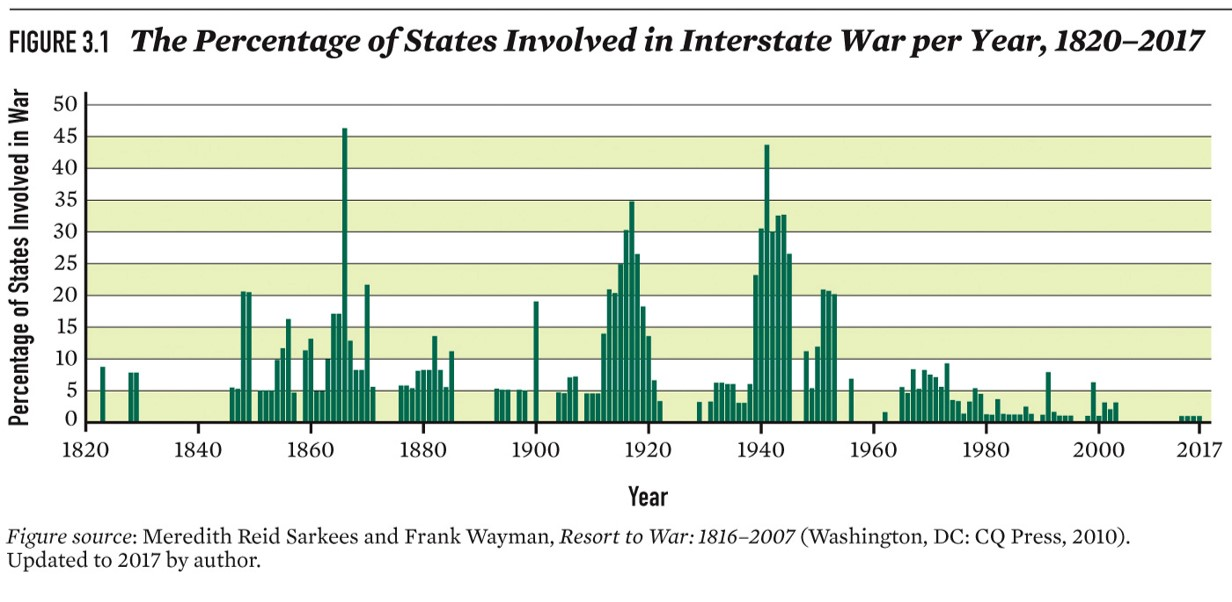
\includegraphics[width=\textwidth,height=0.9\textheight,keepaspectratio]{percentinterstatewar.jpg}
\end{frame}

\begin{frame}{\LARGE Interstate War Statistics} %http://www.systemicpeace.org/conflicttrends.html#fig3
	\centering
	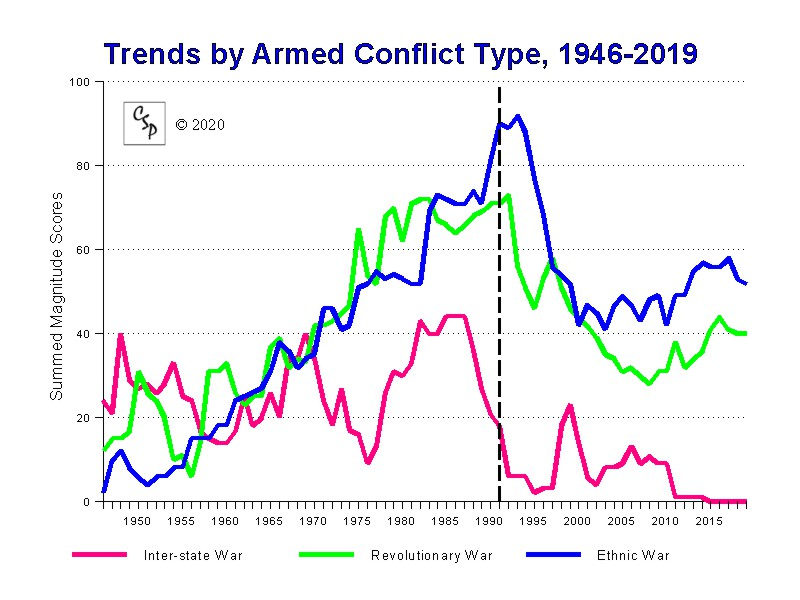
\includegraphics[width=\textwidth,height=0.9\textheight,keepaspectratio]{wartyp19.jpg}
\end{frame}

\begin{frame}{\LARGE Interstate War Statistics} %https://www.prio.org/Projects/Extensions/ConflictTrends/Graphs/?xitem=1631&handler=Project
	\centering
	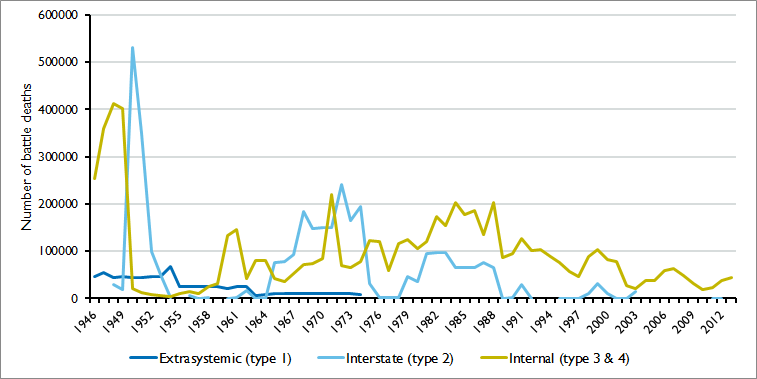
\includegraphics[width=\textwidth]{battledeathnumbers.png}
\end{frame}

\begin{frame} 
	\frametitle{\LARGE{Interstate War Stated Reasons}}
	\begin{itemize}
		\item Territory \pause
		\item National policy \pause
		\item Regime type \pause
		\item Ethnic or religious divisions 		
	\end{itemize}
\end{frame}


\begin{frame} 
\frametitle{\LARGE{Interests, Interactions, and Institutions}}
So, why does interstate war happen?
\begin{itemize}
		\item Conflicting \emph{interests} are necessary, but not sufficient to explain war, as many states have differing interests but few go to war. \pause 
		\item International system lacks \emph{institutions} that can reliably settle disputes and enforce peace (anarchy), but this only permits war without explaining its occurrence. \pause 
		\item However, this environment does permit the \emph{interaction} of bargaining.
\end{itemize}
\end{frame}

\begin{frame} 
\frametitle{\LARGE{Crisis Bargaining}}
	\begin{itemize}
		\item Due to this anarchic system, war is a possible outcome whenever states are trying to divide some good (e.g. territory, policy, regime) in a zero-sum interaction. \pause
		\item \textbf{Crisis bargaining} occurs when at least one state seeks to influence this bargaining by using or threatening force. \pause
		\item Two things determine which deals are acceptable to belligerents during crisis bargaining: the \textbf{costs} and \textbf{likely outcome} of war. 
	\end{itemize}
\end{frame}

\begin{frame} 
\frametitle{\LARGE{Bargaining Model}}
\begin{figure}[ht!]
	\centering
	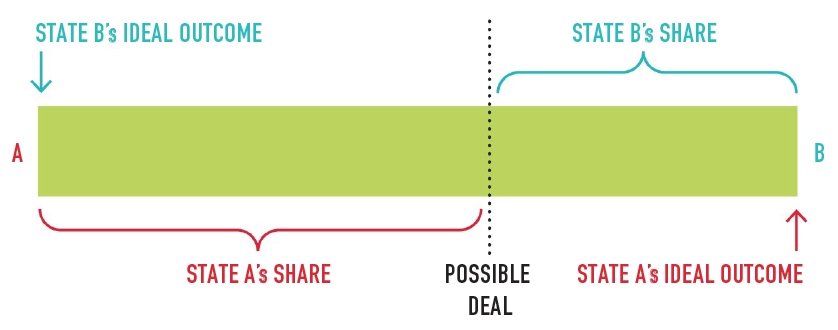
\includegraphics[width=\textwidth,height=0.8\textheight,keepaspectratio]{./barg1.png}
\end{figure}
\end{frame}

\begin{frame} 
\frametitle{\LARGE{Expected War Outcome}}
\begin{figure}[ht!]
	\centering
	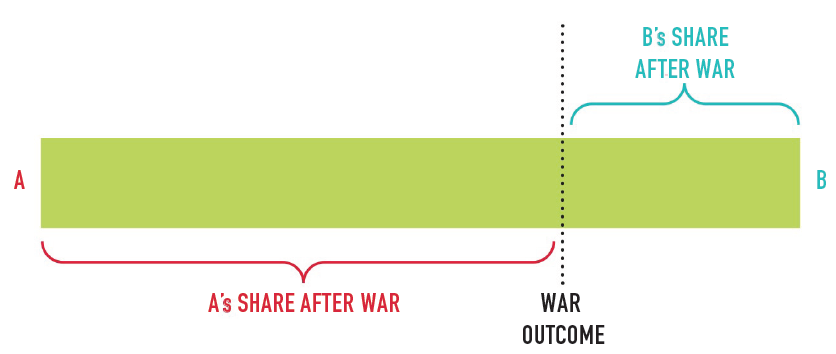
\includegraphics[width=\textwidth,height=0.8\textheight,keepaspectratio]{./barg2.png}
\end{figure}
\end{frame}

\begin{frame} 
	\frametitle{\LARGE{War is Costly!}}
	\begin{itemize}
		\item However, the outcome is not the whole story. \pause
		\item War is costly both in terms of military losses and broader destruction of infrastructure and populations. \pause
		\item We can conceptualize these costs as a negative value, decreasing the total utility a state gets from a war outcome.
	\end{itemize}
\end{frame}

\begin{frame} 
	\frametitle{\LARGE{Bargaining Model: Utility Functions}}
	\begin{itemize}
		\item Say the territory is a divisible good with value 1. \pause
		\item The war outcome is $x$ and costs are $c$. \pause
		\item State A's utility is $U(x) = x -c$ \pause
		\item State B's utility is $U(x) = 1 - x -c$ \pause
		\item These utility functions ensure that the bargaining situation is accurately represented.
	\end{itemize}
\end{frame}

\begin{frame} 
\frametitle{\LARGE{War is Costly!}}
\begin{figure}[ht!]
	\centering
	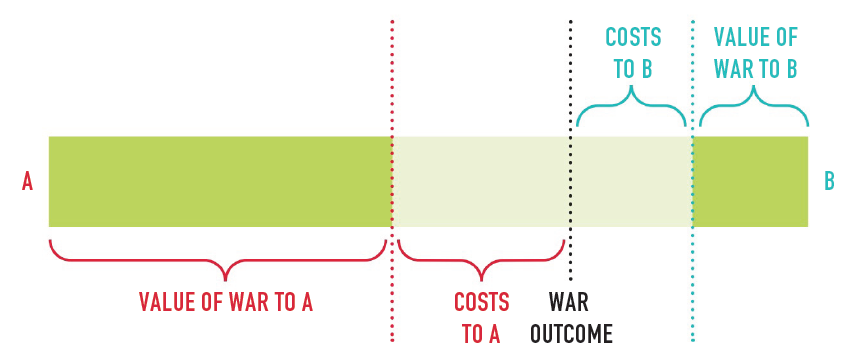
\includegraphics[width=\textwidth,height=0.8\textheight,keepaspectratio]{./barg3.png}
\end{figure}
\end{frame}

\begin{frame} 
\frametitle{\LARGE{Bargaining Range}}
\begin{figure}[ht!]
	\centering
	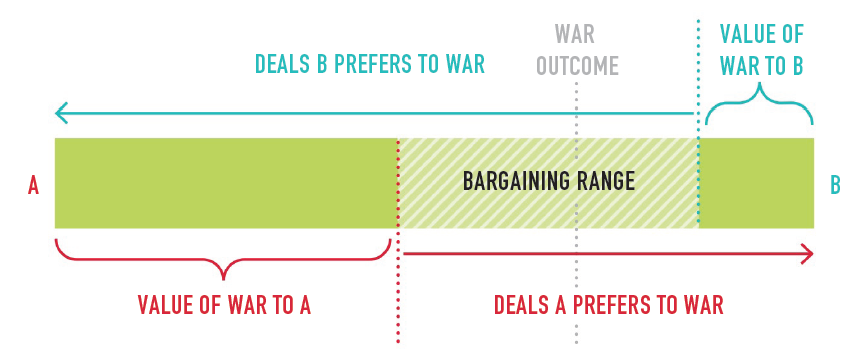
\includegraphics[width=\textwidth,height=0.8\textheight,keepaspectratio]{./barg4.png}
\end{figure}
\end{frame}

\begin{frame} 
	\frametitle{\LARGE{Bargaining Range Implications}}
	\begin{itemize}
		\item The existence of the \textbf{bargaining range} implies a fundamental puzzle of war. \pause
		\item \textbf{Given the existence of a bargaining range, there is always some deal that both sides would prefer to war.} \pause
		\item \textbf{Why do states choose war, given the existence of both the costs of war and the existence of a deal that both sides prefer to war?}
	\end{itemize}
\end{frame}


\begin{frame} 
	\frametitle{\LARGE{Alternative (Failed) Reasons for War}}
	\begin{itemize}
		\item Anarchy/security dilemma \pause
		\item National policy \pause
		\item Regime type \pause
		\item Ethnic or religious divisions \pause	
	\end{itemize}
None of these explain why war occurs, given the presence of a bargaining range.
\end{frame}

\begin{frame} 
\frametitle{\LARGE{Bargaining Model}}
So, how does the bargaining model explain war? Stay tuned...
\end{frame}

\end{document}
